\newpage
\section{Auswertung}
Für den ersten Teil der Auswertung wurde der Entladevorgang eines Kondensators untersucht.\\
Dabei wurde die Kondensatorspannung und die Zeit seit Beginn des Entladevorgangs gemessen.
Diese Messwerte finden sich in der Tabelle \ref{tab:1} und grafisch dargestellt in Abbildung \ref{img:1}.\\
In der Abbildung wurde der Logarithmus der Kondensatorspannung geteilt durch die angelegte Spannung gegen die Zeit aufgetragen.\\
Zusätlich ist dort noch ein linearer Fit auf die halblogarithmischen Messwerten abgebildet. Dieser hat die Form:
\begin{equation*}
    \log{\frac{U_C}{U_0}}= -\frac{1}{RC_1}\cdot t +n
\end{equation*}
Wobei $RC_1= \SI{0.0082(4)}{\second}$ und $\SI{-0.16694(14582)}{}$ gilt. Dabei ist $RC$ hier auch der zu bestimmende Wert der Zeitkonstanten.

\begin{figure}[h]
    \centering
    \includegraphics[width=0.6\textwidth]{build/plots/plot0.pdf}
    \caption{Ein linearer Fit auf die halblogarithmischen dargestellten Messwerte von Spannung und Zeit.}
    \label{img:1}
\end{figure}

\begin{table}[h]
    \centering
    \small
    \begin{tabular}{S [table-format=2.3] S [table-format=2.3] S [table-format=2.3]}
        \toprule
        {$U_C \mathbin{\scalebox{1.5} / }\si{\volt}$} & {$\log{\frac{U_C}{U_0}} $} & {$t \mathbin{\scalebox{1.5} / }\si{\second}$}\\
        \midrule
        0.620 & -0.478 & 0.000\\
        0.520 & -0.654 & 0.002\\
        0.420 & -0.868 & 0.004\\
        0.340 & -1.079 & 0.006\\
        0.290 & -1.238 & 0.008\\
        0.240 & -1.427 & 0.010\\
        0.200 & -1.609 & 0.012\\
        0.170 & -1.772 & 0.014\\
        0.125 & -2.079 & 0.016\\
        0.100 & -2.303 & 0.018\\
        0.085 & -2.465 & 0.020\\
        0.070 & -2.659 & 0.022\\
        0.060 & -2.813 & 0.024\\
        0.050 & -2.996 & 0.026\\
        0.040 & -3.219 & 0.028\\
        0.030 & -3.507 & 0.030\\
        0.020 & -3.912 & 0.032\\
        0.010 & -4.605 & 0.036\\
        0.001 & -6.908 & 0.046\\
        \bottomrule
    \end{tabular}
\caption{Die Messwerte der abfallenden Kondensatorspannung in Abhängigkeit von der Zeit. Zusätzlich noch die für das Pslotten verwendeten logarithmierten Spannungswerte.}
\label{tab:1}
\end{table}


\noindent Ein alternativer Weg zur Bestimmung von $RC$ ist die Frequenzabhängigkeit der Kondensatorspannung zu messen und auf diese Messwerte wieder eine Ausgleichsrechnung auszuführen.\\
Die dazu gehörigen Messwerte sind in der Tabelle \ref{tab:2} zu finden.\\
Die Ausgleichfunktion hat dabei folgende Form und die Rechnung führt zu folgendem Ergebnis:
\begin{align*}
    U_C(\nu)&=\frac{A}{\sqrt{1+(RC_2)^2\cdot \nu^2}}\\
    RC_2&=\SI{0.0067(2)}{\second}\\
    A&=\SI{0.3220(31)}{\volt}
\end{align*}

\noindent Diese Funktion lässt sich zusammen mit den Messwerten in Abbildung \ref{img:2} dargestellt finden.

\begin{figure}[H]
    \centering
    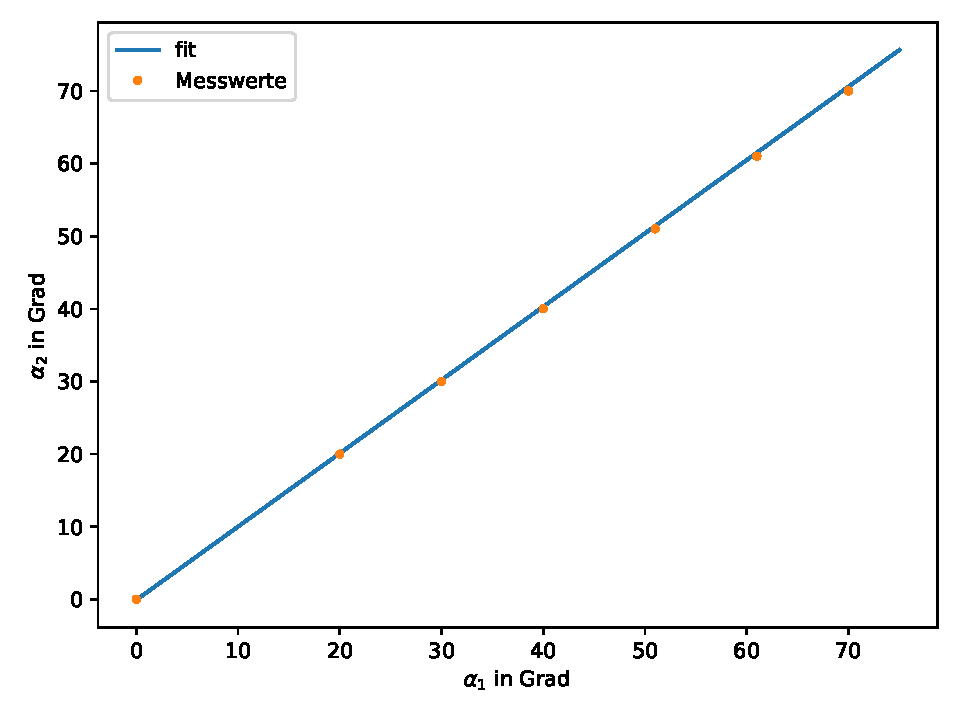
\includegraphics[width=0.6\textwidth]{build/plots/plot1.pdf}
    \caption{Die Messwerte der Kondensatorspannung aufgetragen gegen die logarithmierte Frequenz. Zusätzlich noch die Fit-Funktion. }
    \label{img:2}
\end{figure}
\begin{table}[h]
    \centering
    \small
    \begin{tabular}{S [table-format=2.3]  S [table-format=5.3]}
        \toprule
        {$U_C \mathbin{\scalebox{1.5} / }\si{\volt}$}  & {$\nu \mathbin{\scalebox{1.5} / }\si{\hertz}$}\\
        \midrule
        0.320 & 10.000 \\
        0.330 & 25.000 \\
        0.305 & 50.000 \\
        0.280 & 75.000 \\
        0.260 & 100.000\\
        0.190 & 200.000\\
        0.145 & 300.000\\
        0.100 & 500.000\\
        0.068 & 750.000\\
        0.052 & 1000.000\\
        0.021 & 2500.000\\
        0.011 & 5000.000\\
        0.005 & 10000.000\\
        0.004 & 15000.000\\
        0.003 & 20000.000\\
        0.001 & 50000.000\\
        \bottomrule
    \end{tabular}
\caption{Die Messwerte der Spannung in Abhängigkeit von der Frequenz.}
\label{tab:2}
\end{table}


\noindent Die letzte Methode zur Bestimmung der Zeitkonstante ist die über die Phasenverschiebung.\\ 
Dabei wird die Phasenverschiebung der Kondensatorspannung von der angelegten Spannung, in Abhängigkeit von der Erzeugerfrequenz gemessen.
Da die Phasenverschiebung hier nicht direkt gemessen werden kann wird der Laufzeitunterschied $a$ gemessen und daraus die Verschiebung bestimmt.
Dafür wird die Gleichung $\phi= a\cdot\nu\cdot 2\pi$ genutzt.\\
Diese Werte der Phasenverschiebung und des Laufzeitunterschieds sind in Tabelle \ref{tab:3} dargestellt.\\\\
\noindent Um nun aus der Phasenverschiebung die Zeitkonstante zu bestimmen muss eine Ausgleichsrechnung mit einem Arkustangens durchggeführt werden.\\
Diese Rechnung führt zu folgendem:
\begin{align*}
    \phi(\nu)&=B\cdot \arctan(RC_3 \cdot \nu)\\
    B&=\SI{0.9253(128)}{}\\
    m&=\SI{0.00704(61)}{\second}
\end{align*}
Zu finden ist dies in Abbildung \ref{img:3}.

\begin{figure}[H]
    \centering
    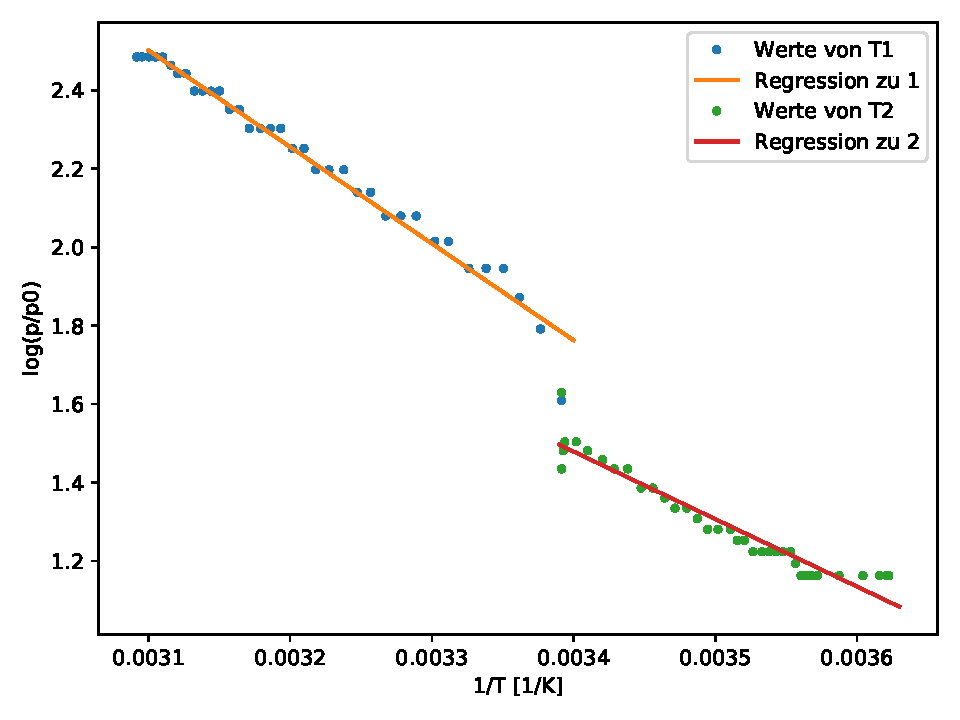
\includegraphics[width=0.6\textwidth]{build/plots/plot2.pdf}
    \caption{Die aus den Messwerten errechnete Phasenverschiebung aufgetragen gegen die logarithmierte Frequenz. Zusätzlich noch die Fit-Funktion in Form eines Arkustangens. }
    \label{img:3}
\end{figure}

\begin{table}[h]
    \centering
    \small
    \begin{tabular}{S [table-format=1.3] S [table-format=1.3] S [table-format=5.3]}
        \toprule
        {$a \mathbin{\scalebox{1.5} / }\si{\micro\second}$} & {$\phi \mathbin{\scalebox{1.5} / }\si{\radian}$} & {$f \mathbin{\scalebox{1.5} / }\si{\hertz}$}\\
        \midrule
        1.000 & 0.157 & 25.000\\
        1.200 & 0.377 & 50.000\\
        0.900 & 0.565 & 100.000\\
        0.600 & 0.942 & 250.000\\
        0.380 & 1.194 & 500.000\\
        0.270 & 1.272 & 750.000\\
        0.210 & 1.319 & 1000.000\\
        0.150 & 1.414 & 1500.000\\
        0.100 & 1.257 & 2000.000\\
        0.058 & 1.458 & 4000.000\\
        0.040 & 1.508 & 6000.000\\
        0.029 & 1.458 & 8000.000\\
        0.024 & 1.508 & 10000.000\\
        0.015 & 1.414 & 15000.000\\
        0.011 & 1.382 & 20000.000\\
        \bottomrule
    \end{tabular}
\caption{Der Laufzeitunterschied der beiden Spannungen, die daraus errechnete Phasenverschiebung und die damit korrespondierenden Frequenzen.}
\label{tab:3}
\end{table}

\noindent Wenn nun die Messwerte Spannungen in Abhängigkeit von der Frequenz und die damit in der dritten Messreihe korrespondierenden Phasenverschiebungen herausgesucht werden, lassen sich die in Tabelle \ref{tab:4} dargestellten Messwertpaare finden.
Dabei wurden nur Werte genutzt für die identische Frequenzen in beiden Messreihen existieren.\\



\noindent Diese Messwerte lassen sich in einem Polardiagramm, wie in Abbildung \ref{img:4} darstellen. 
Dabei wird auch noch die Funktion \ref{eqn:12} mit $RC_1$ eingezeichnet.
\begin{figure}[H]
    \centering
    \includegraphics[width=0.6\textwidth]{build/plots/plot3.pdf}
    \caption{Ein Polardiagramm der Messwerte.}
    \label{img:4}
\end{figure}

\begin{table}[h]
    \centering
    \small
    \begin{tabular}{S [table-format=1.5] S [table-format=1.6] }
        \toprule
        {$U \mathbin{\scalebox{1.5} / }\si{\volt}$} & {$\phi \mathbin{\scalebox{1.5} / }\si{\radian}$} \\
        \midrule
        0.33    & 0.15708  \\
        0.305   & 0.376991 \\
        0.26    & 0.565487 \\
        0.1     & 1.19381  \\
        0.068   & 1.27235  \\
        0.052   & 1.31947  \\
        0.00505 & 1.50796  \\
        0.004   & 1.41372  \\
        0.003   & 1.3823   \\
        \bottomrule
    \end{tabular}
\caption{Die Spanungen und Phasenverschiebungen die im Polardiagramm eingezeichnet sind.}
\label{tab:3}
\end{table}
